\documentclass[11pt,pdftex,portrait,letterpaper]{article}
\usepackage[hdivide={1in,*,1in},
            vdivide={1in,*,1in},
%            showframe
            ]{geometry}

% Standard packages
\usepackage[T1]{fontenc}
\usepackage{graphicx}
\usepackage{longtable}
\usepackage{acronym}
\usepackage{verbatim}
\usepackage{subfigure}
\usepackage{fancyhdr}
\pagestyle{fancy}
\usepackage{listings}
\usepackage{color}
\usepackage{lastpage}
\usepackage{caption}

% Fonts
%\usepackage{libertine}	% Libertine (the main font)
%\usepackage[lcgreekalpha]{libertinust1math}	% Libertine (as the math font)
\usepackage[varl]{inconsolata}	% A monospace font similar to Consolas. The varl option makes the lowercase l look different than a numeral 1.

% Last packages
\usepackage[hidelinks]{hyperref}	% Hyperlinks

% Modify parameters of Listings
\definecolor{lstgreen}{rgb}{0,0.6,0}
\definecolor{lstgray}{rgb}{0.4,0.4,0.4}
\lstset{ 
	language=C,
	basicstyle=\ttfamily\scriptsize,
	numbers=left,
	numberstyle=\footnotesize,
	keywordstyle=\color{blue},
	identifierstyle=\color{black},
	commentstyle=\color{lstgreen},
	stringstyle=\color{lstgray},
	stepnumber=1,
	numbersep=10pt,
	backgroundcolor=\color{white},
	frame=single,
	captionpos=b,
	breaklines=true,
	breakatwhitespace=false,
	tabsize=2,
	showstringspaces=false
}

% Default margins are too wide all the way around. Reset them here
\setlength{\topmargin}{-.5in}
\setlength{\textheight}{9in}
\setlength{\oddsidemargin}{0in}
\setlength{\textwidth}{6.5in}

\lhead{ECEN 220}
\chead{GPIO Project 1}
\rhead{\thepage\ of \pageref{LastPage}}
\lfoot{\small{University of Nebraska--Lincoln}}
\cfoot{}
\rfoot{\small{Department of Electrical \& Computer Engineering}}
\renewcommand{\footrulewidth}{0.5pt}




\begin{document}

\vspace*{30ex}
\begin{center}

\textbf{GPIO Project 1}\\

\vspace{4ex}
ECEN 220: Introduction to Embedded Systems\\
University of Nebraska--Lincoln\\
February 24, 2021

\vspace{4ex}
Name: David Perez\\

\end{center}


\pagebreak
\tableofcontents
%\pagebreak
%\listoffigures
%\addcontentsline{toc}{section}{{\bf List of Figures}}
\pagebreak


\section{Introduction}

The intention behind this project was to gain an understanding of the atmega328p GPIO (general purpose input output) registers. In the subsequent pages, there is source code and square waves to demonstrate how these  registers behave in ways such as their execute time, creating delays, and even debouncing their pins.
 
\section{Program Description}

The purpose of program 1 is simply to introduce how to make a pin an output in order to allow an led to blink as fast as possible. The second programs intention was to print to the serial monitor each iteration that the loop was on and to take note of each instructions execution time. The third program on the other hand was nearly opposite of the first as its intended to create a delay that lasts X amount of milliseconds everytime the function is called. And finally, the final program introduces the concept of pin debouncing and how there is noise when reading  signals and attempts to block out that noise via the delay function from program 3. Also, keep in mind that the source code for these programs will be located in the appendix section of this pdf.

\subsection{Program 1}

The loop is taking 9 cycles to complete which seems pretty reasonable to me. The frequency also seems fairly accurate because each period takes 2.7MHz / 375 ns to complete is 1/10 the clock speed that the MCU is running at.

 The square wave is not showing a 50 percent duty cycle. I believe this is occurring because the led is off for a longer period than it is on which  results from it having to return to the beginning of the loop.
 
 If you wanted to create a 50 percent duty cycle you could insert a delay after you set PB1 high and with enough tinkering you could offset the lopsidedness that arises from the MCU having to return to the beggining of the loop. 

% This is how you add a figure
\begin{figure}[h]
\centering
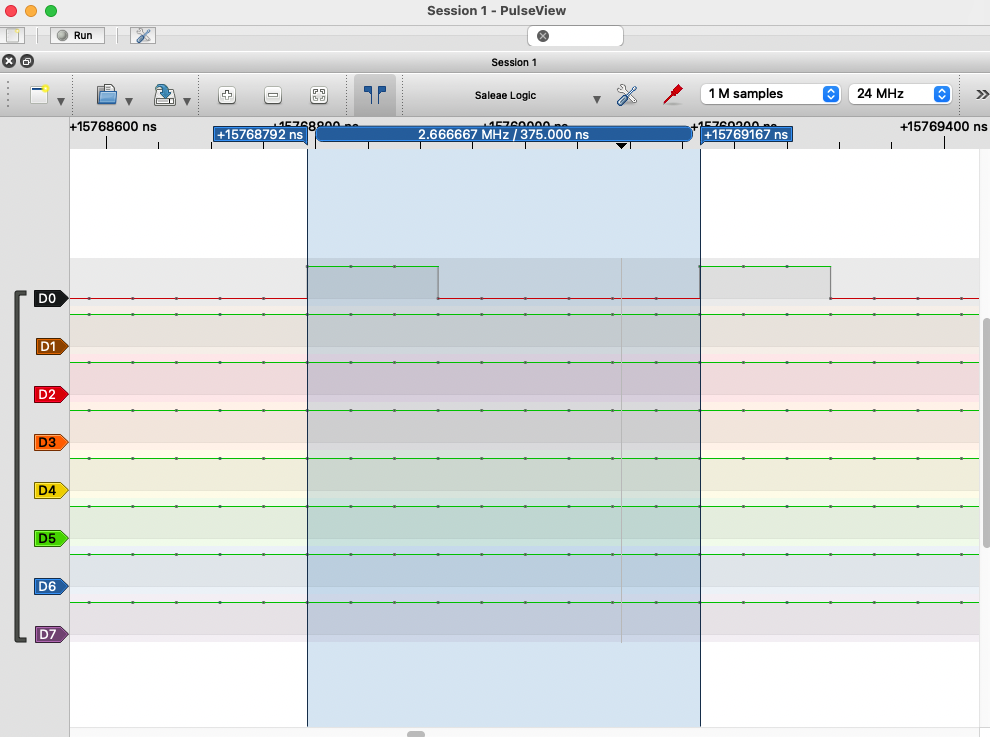
\includegraphics[width=0.6\textwidth]{./PG1_logicAnalyzer}	% The .png file will be used to make the figure here, and is in the same directory as this .tex file
\caption{Screen Capture of program 1 square wave function}
\label{f:fig1}	% labels must come after the caption
\end{figure}

\pagebreak


\subsection{Program 2}

As mentioned before the intent of this program was to caculate the execution time of some basic gpio commands on the atmega329p MCU. Figure 2 below shows that it took just about 20ms to set PB1 pin high, write a string to the serial monitor, then set PB1 low again.
In figure 3, it displays a chunk of the code used to perform this action and how it was outputted onto the serial monitor.

Also take note that square wave shows that once the pin is turned high it takes roughly 19.77 ms to execute the sprintf and Serial.write functions. On the contrary it only takes about 1 microsecond to turn the pin low.




\begin{figure}[h]
	\centering
	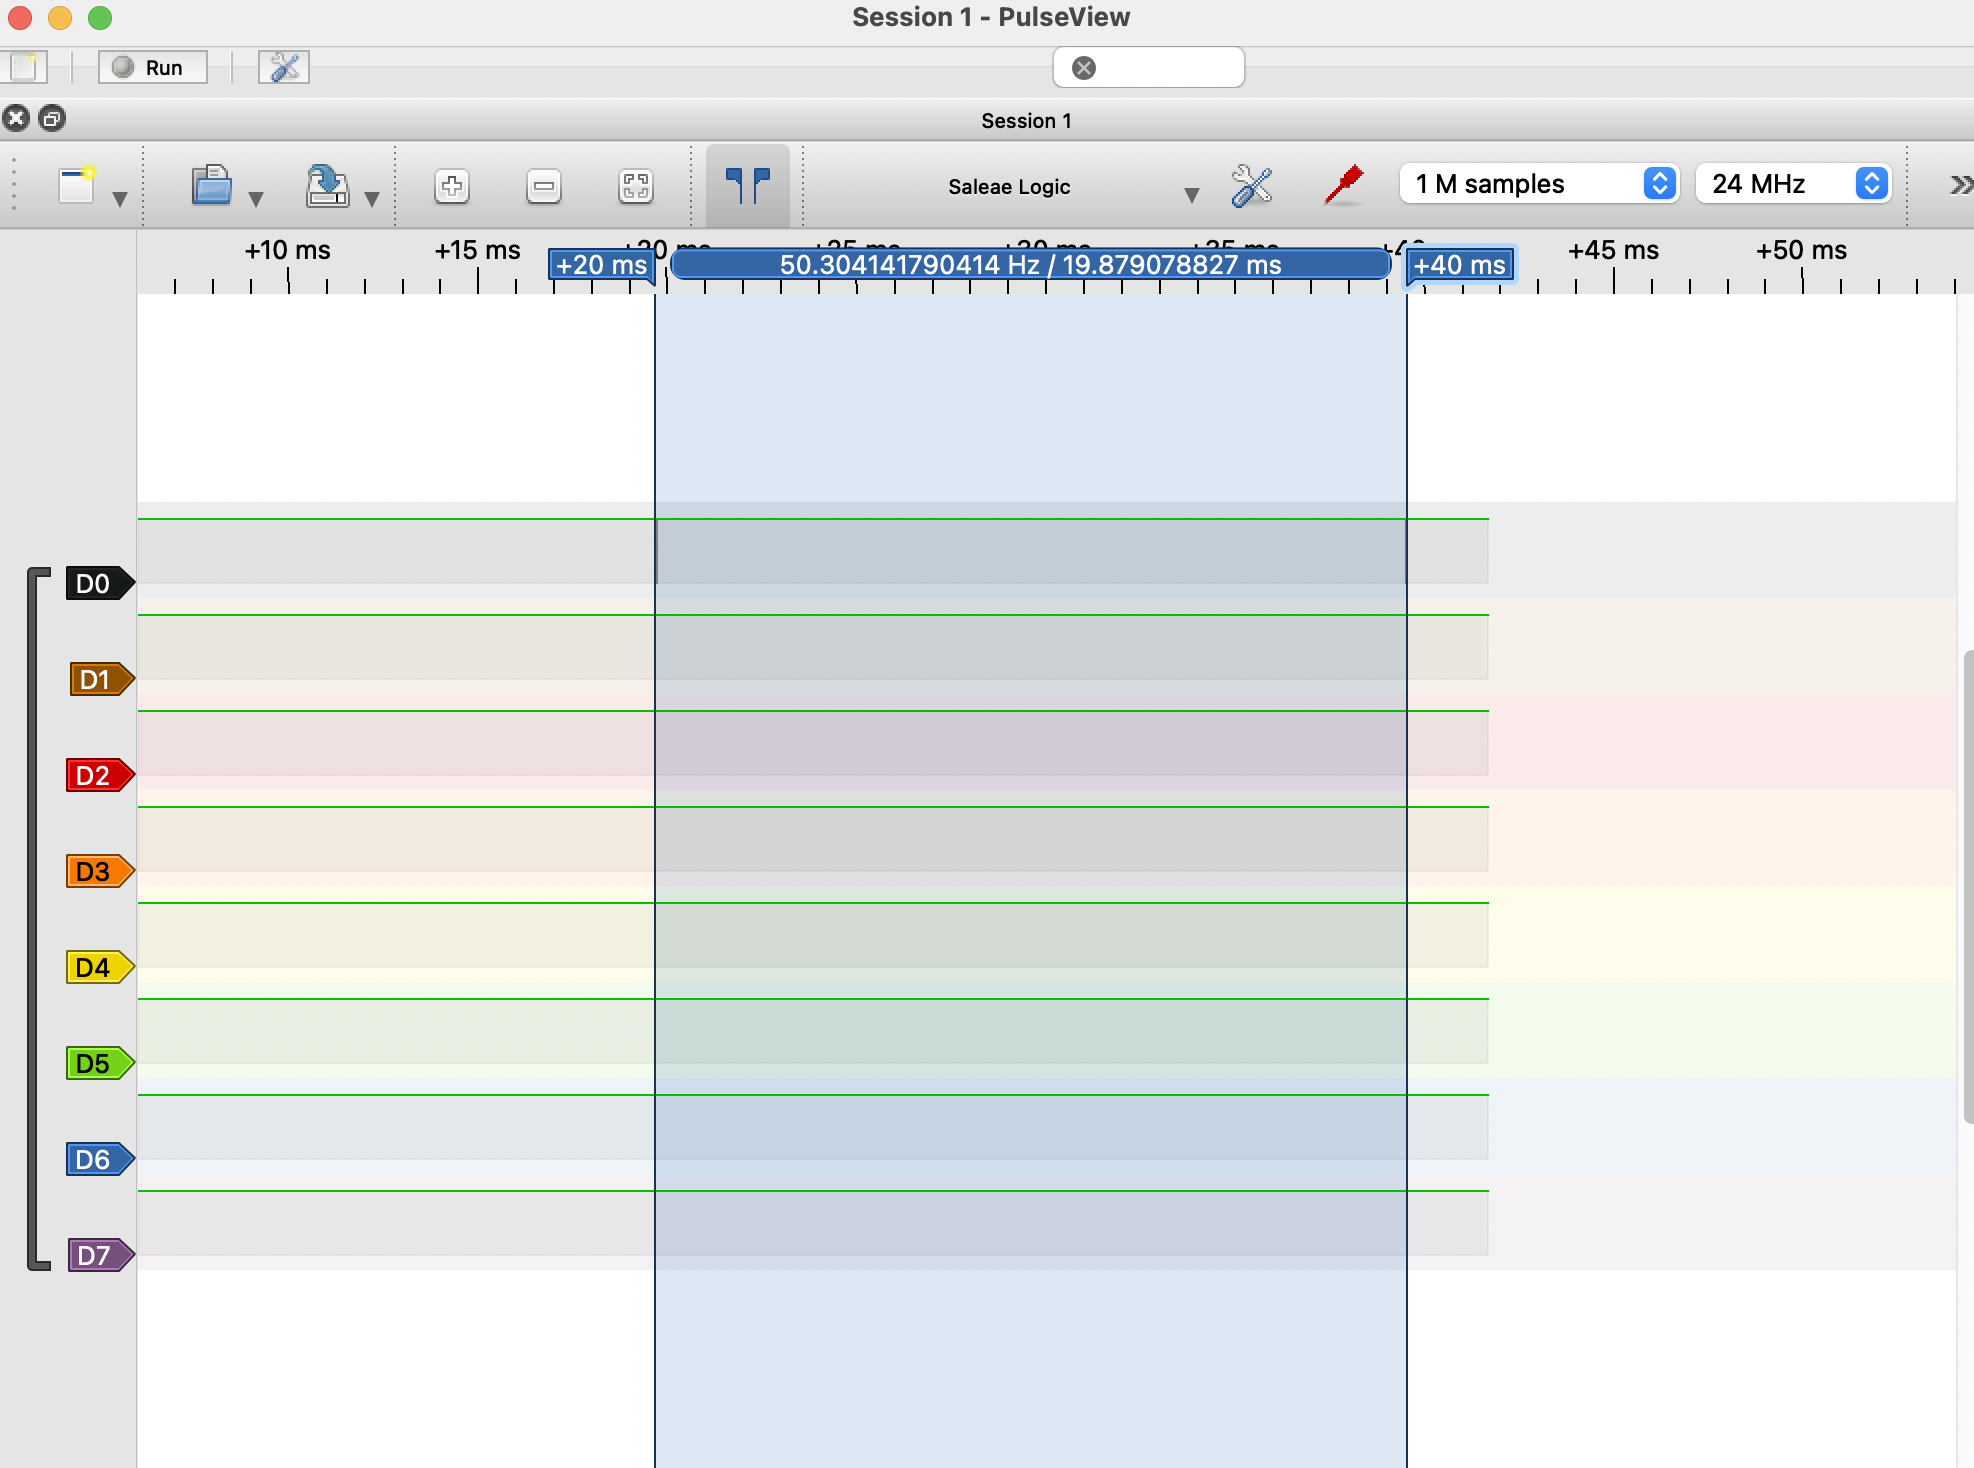
\includegraphics[width=0.6\textwidth]{./PG2_logicAnalyzer_1}	% The .png file will be used to make the figure here, and is in the same directory as this .tex file
	\caption{Screen Capture of program 2 square wave function}
	\label{f:fig1}	% labels must come after the caption
\end{figure}
\begin{figure}[h]
	\centering
	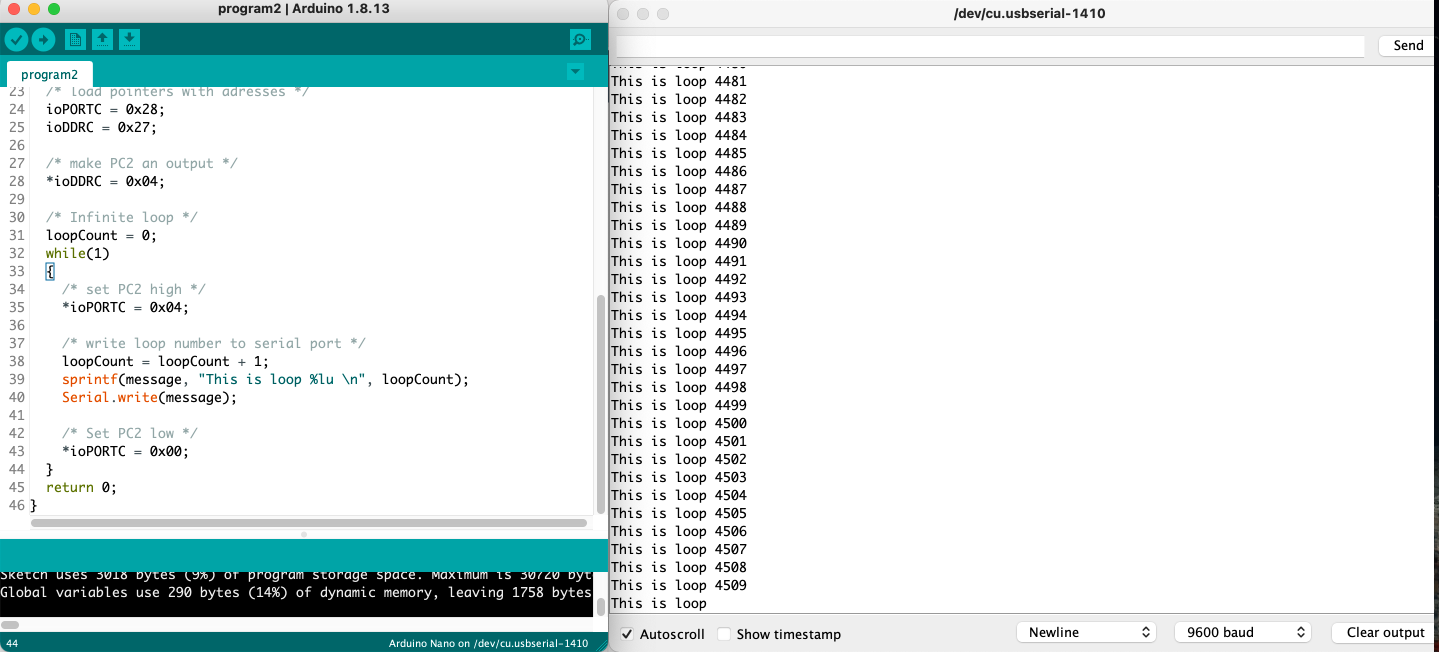
\includegraphics[width=0.6\textwidth]{./PG2_serialMonitor}	% The .png file will be used to make the figure here, and is in the same directory as this .tex file
	\caption{Screen Capture of program 2 square wave function}
	\label{f:fig1}	% labels must come after the caption
\end{figure}

Another important thing to understand is that executing the serial functions are very time consuming for the MCU. When adding only 9 characters onto the message string it took the MCU another 10 ms totaling roughly 30.18 ms versus the 19.77 ms without the extra characters. This is shown in figure 4.
\begin{figure}[h]
	\centering
	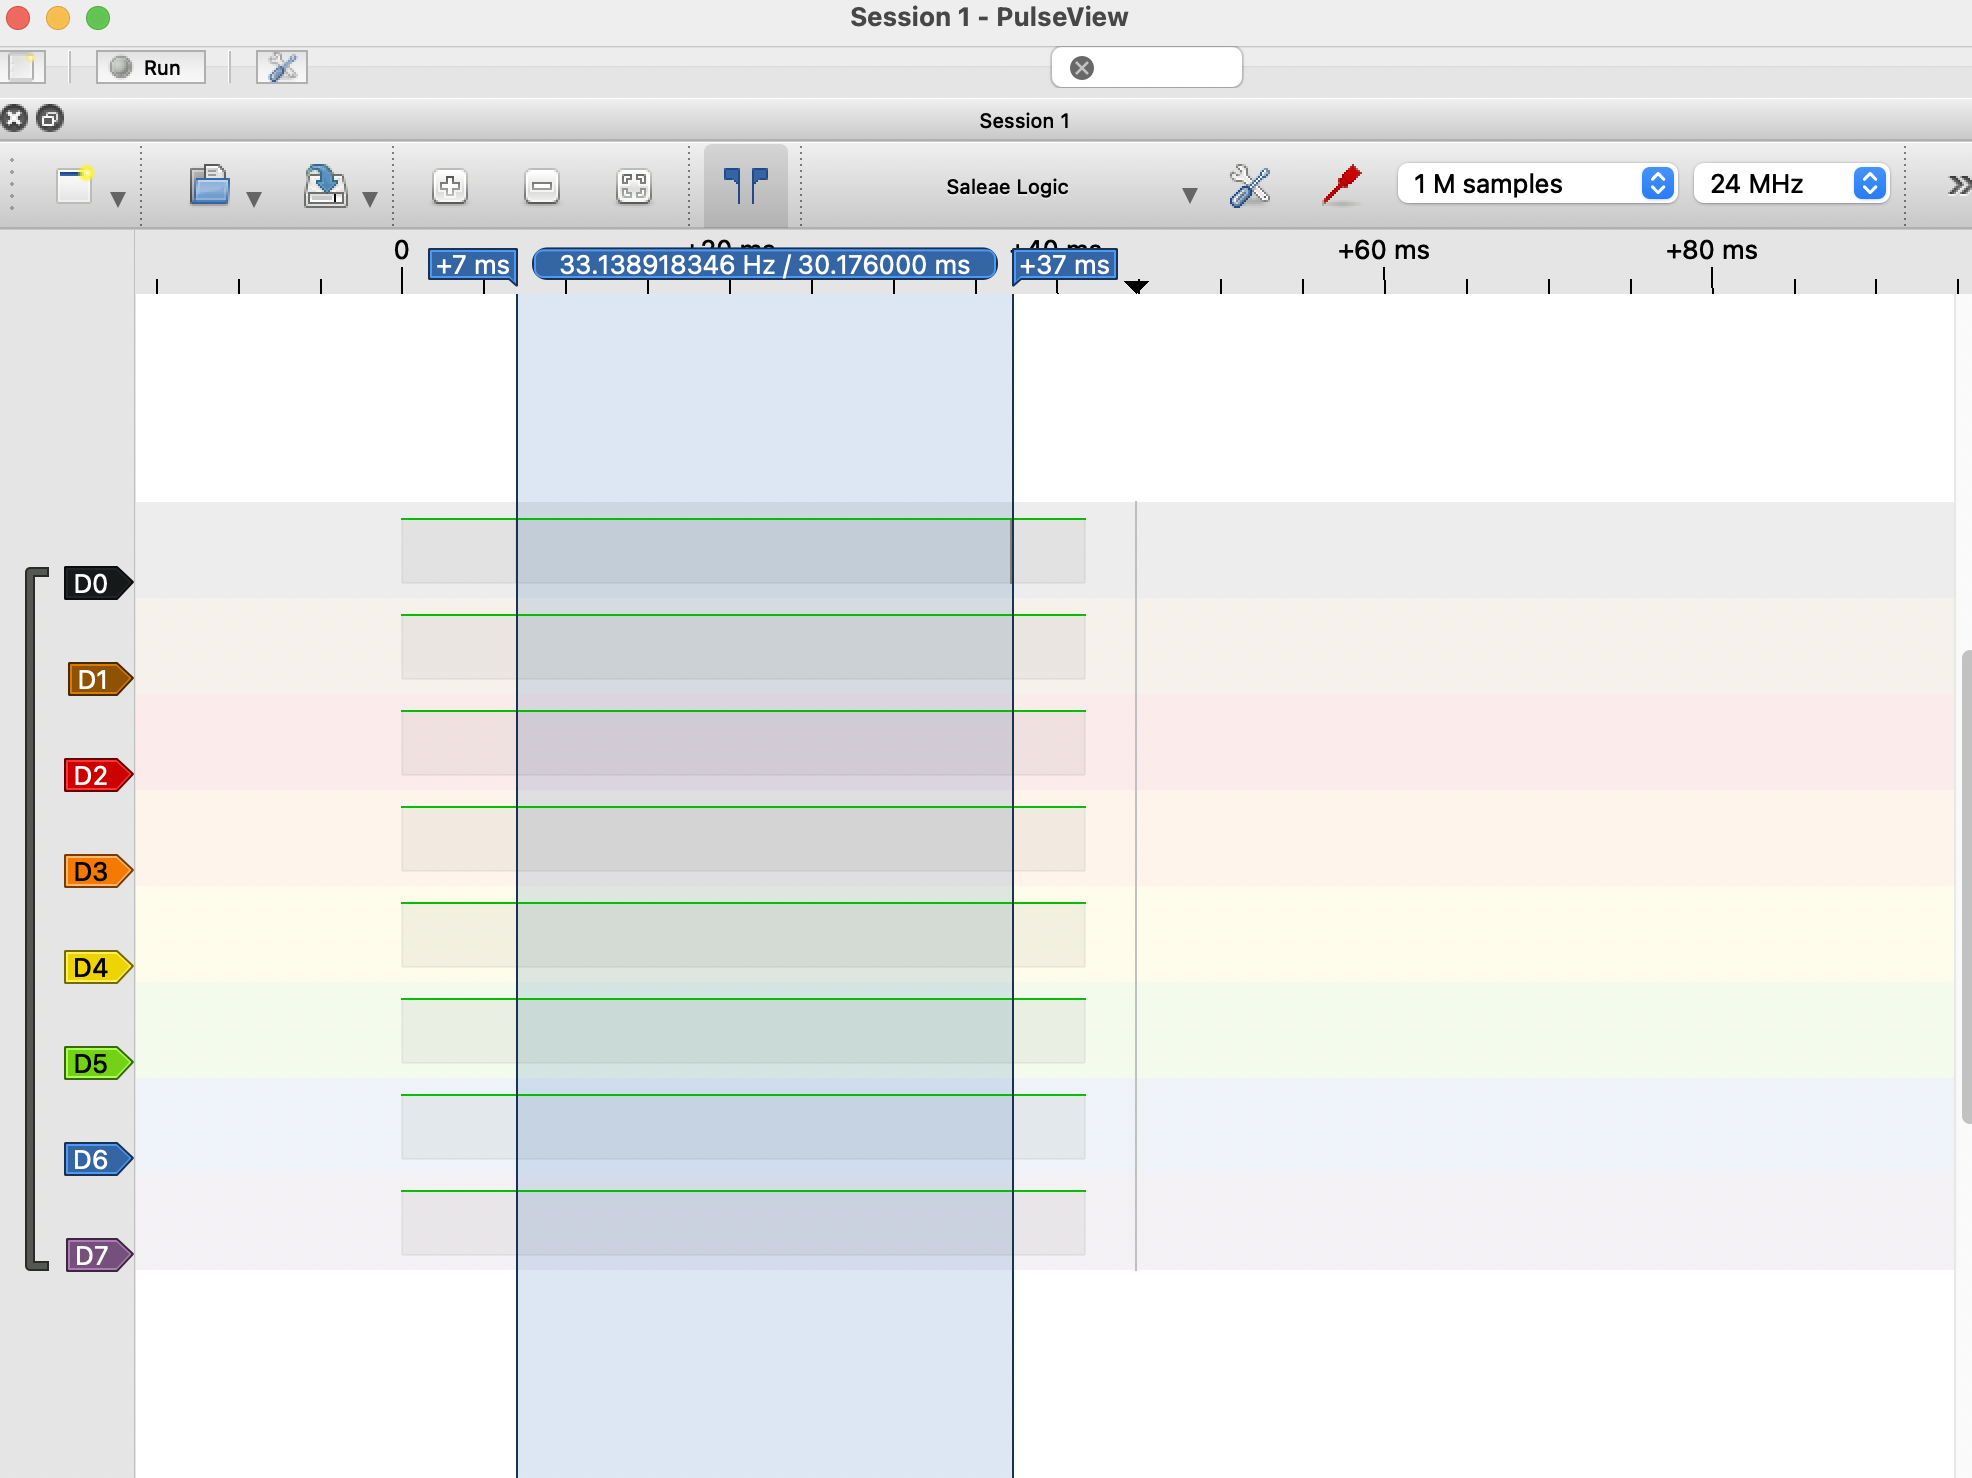
\includegraphics[width=0.6\textwidth]{./PG2_logicAnalyzer_2}	% The .png file will be used to make the figure here, and is in the same directory as this .tex file
	\caption{Screen Capture of program 2 delayed square wave}
	\label{f:fig1}	% labels must come after the caption
\end{figure}

\pagebreak

\subsection{Program 3}

In order to get a proper millisecond delay function I used a value of 373 that I would then multiply by the arguments passed into my "myHardDelay" function.

The value that resulted from the multiplication of 373 and the parameter, was passed into a variable called delayCount that was made volatile in order to prevent the delay from being optimized by the compiler.

When “1” is inserted into the function, the period (from rising edge to falling edge) is 2.016 ms. Thus the delay is roughly 1ms, that is 1ms when the pin is turned high and another 1ms when the delay is called again, after turning the pin low . When it comes to inserting 50 into the function the delay gets only slightly more inaccurate. The delay function took 50.15ms to execute when 50 was an argument to the function.

I found that the maximum delay would be roughly 5,757,329 which I derived from taking the maximum decimal digit a 32 bit number could hold then dividing by my N which is 373.
\begin{figure}[h]
	\centering
	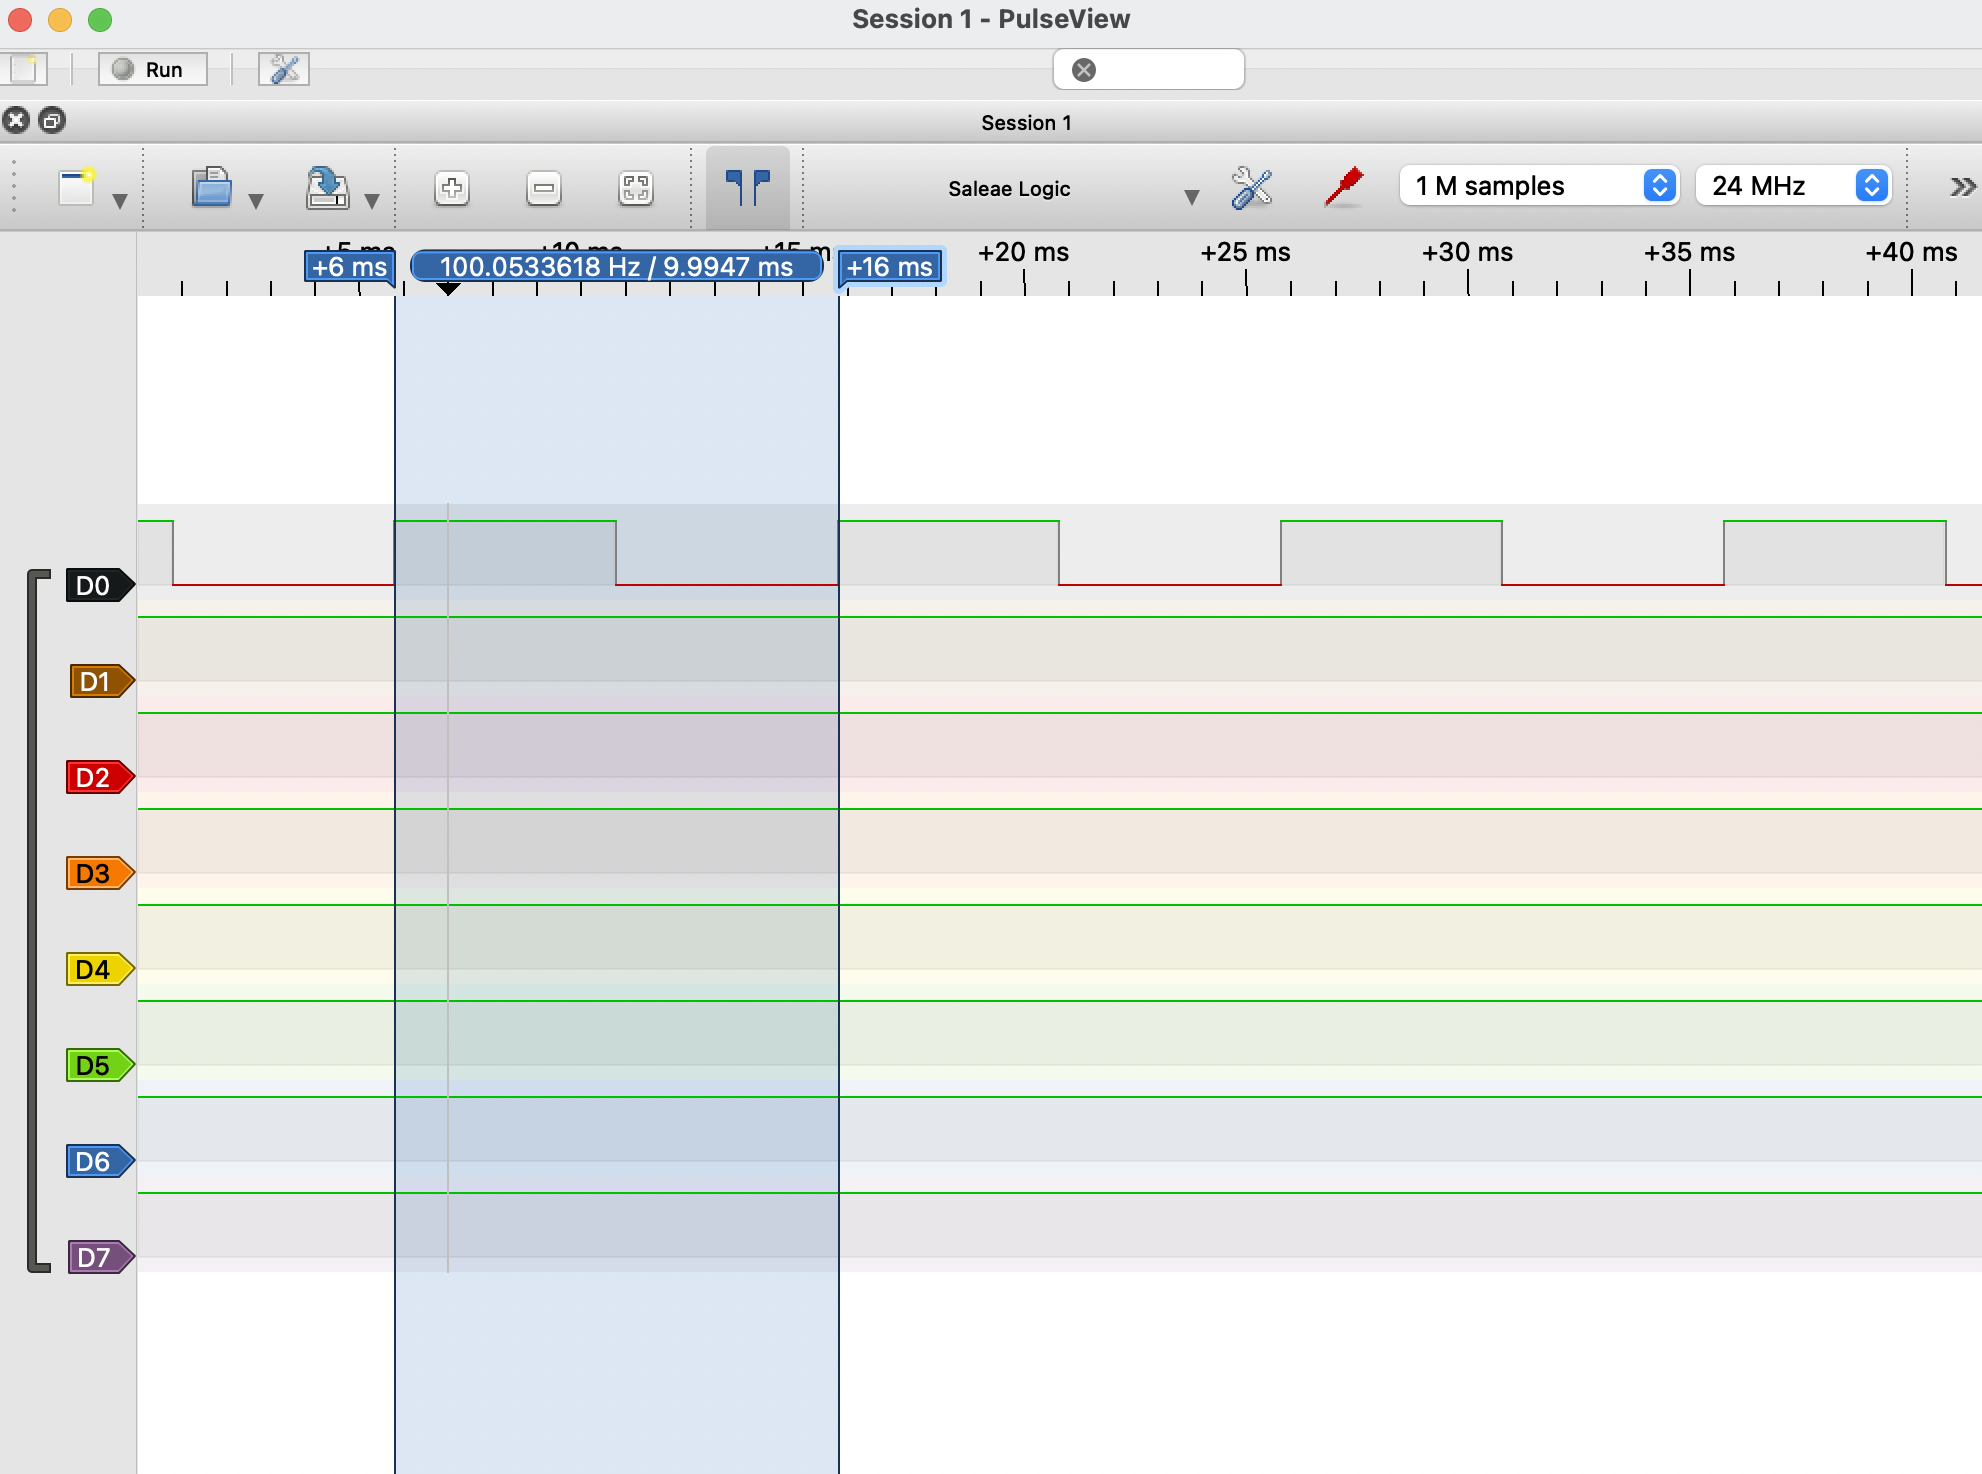
\includegraphics[width=0.6\textwidth]{./PG3_logicAnalyzer}	% The .png file will be used to make the figure here, and is in the same directory as this .tex file
	\caption{Screen Capture of program 3 100Hz square wave}
	\label{f:fig1}	% labels must come after the caption
\end{figure}
\pagebreak


\subsection{Program 4}

Without debouncing the pin it was apparent that there was indeed a need to debounce pins especially in the case of the push button. Without a delay signal read, the serial monitor would display presses even after the button had already been released. 

The delay I chose is roughly 68 milliseconds. I chose this value because I had to take into account the time it took for the serial monitor to actually output my stings. If I had increased that delay too much more I’d also run into the problem of the serial monitor showing a button not pressed string when the button was pressed and would even exclude the bouncing signal.

I found 68 milliseconds to be just about the perfect delay where it would display the proper status of the button press. When decreasing only a few milliseconds the serial monitor would show multiple lines declaring the button was pressed when it wasn’t. 


\section{Conclusion}

Through each program there were some very good fundamental takeaways. From the first program one could gain an understanding of how gpio registers work. Continuining to program 2 I was able to understand the impact that certain commands have and ones like the Arduino's "Serial.write" take significantly longer than simply changing a register value. An important takeaway from program 3 is simply the architecture of how a delay function is wrote. Combining the delay in program 3 with the debouncing pins and with program 4 you could accuratley read changing values from a simple small electronic button.

\pagebreak

\section{Appendix}

%Here is an example of how to add good-looking code snippets using a 'listing' 
\begin{lstlisting}[caption={Program 1}, label=l:programx]
#include <stdint.h>

/** GLOBAL Variables */
volatile uint8_t* pDDRB;
volatile uint8_t* pPORTB;


/* Main Function */

int main(void)
{
	/* Define our pointers to the GPIO registers */
	pDDRB = 0x24;
	pPORTB = 0x25;
	
	/* Set PB1 as an output with the DDRB register */
	*pDDRB = 0x02; // 0x01 = 0b00000010
	
	while(1)
	{
		/* Set PB1 high */
		*pPORTB = 0x02;
		
		/* Clear PB1 low */
		*pPORTB = 0x00;
	
	}	
}

\end{lstlisting}

\begin{lstlisting}[caption={Program 2}, label=l:programx]

	/** Includes **/
	// arduino wiring library (contains serial.begin() and serial.write()
	#include <Arduino.h>
	#include <stdint.h>
	#include <stdio.h>  // contains sprintf() and snprintf()
	
	/** Global Variable **/
	volatile uint8_t* ioPORTC;
	volatile uint8_t* ioDDRC;
	uint32_t loopCount;
	char message[80];
	
	int main() 
	{
		/* initialize the arduino wiring library */
		init();
		
		/* inintialize the serial port with a band of 9600 bits per second */
		Serial.begin(9600);
		
		/* load pointers with adresses */
		ioPORTC = 0x28;
		ioDDRC = 0x27;
		
		/* make PC2 an output */
		*ioDDRC = 0x04;
		
		/* Infinite loop */
		loopCount = 0;
		while(1)
		{
			/* set PC2 high */
			*ioPORTC = 0x04;
			
			/* write loop number to serial port */
			loopCount = loopCount + 1;
			sprintf(message, "This is loop %lu \n", loopCount);
			Serial.write(message);
			
			/* Set PC2 low */
			*ioPORTC = 0x00;
		}
		return 0;
	}
	
\end{lstlisting}

\begin{lstlisting}[caption={Program 3}, label=l:programx]

#include <stdint.h>

volatile uint32_t i;
volatile uint8_t* pDDRB;
volatile uint8_t* pPORTB;
volatile uint32_t delayCount;

void myHardDelay(uint32_t delayInMsec);

int main()
{
	
	//load pointers with addresses
	pDDRB = 0x24;
	pPORTB = 0x25;
	
	
	//make PB1 an output
	*pDDRB = 0x02; // 0x01 = 0b00000010
	
	
	while(1)
	{
		
		//set PB1 high then delay for 1 milliseconds
		*pPORTB = 0x02;
		
		//delay 1 millisecond
		myHardDelay(1);
		
		//set PB1 low then delay for 1 milliseconds
		*pPORTB = 0x00;
		myHardDelay(1);
	}
}
void myHardDelay(uint32_t delayInMsec)
{
	delayCount = delayInMsec * 373;
	for(i=0;i <delayCount; i++){	
	}
}
	
\end{lstlisting}

\begin{lstlisting}[caption={Program 4}, label=l:programx]
	
/* Includes */
#include <Arduino.h>
#include <stdint.h>
#include <stdio.h>

/** GLOBAL Variables */
volatile uint8_t* pPINB;
volatile uint8_t* pDDRB;
volatile uint8_t* pPORTB;




/* Function Declarations */
int8_t debouncePin(volatile uint8_t* mmrPINx, uint8_t bitToRead);
void myHardDelay(uint32_t delayInMsec);


// Main Function
int main(void)
{
	// Initialize the Arduino Wiring Library
	init();
	//Initialize the serial port with a band of 9600 bits per second
	Serial.begin(9600);
	
	/* Define our pointers to the GPIO registers */
	pPINB = 0x23;
	pDDRB = 0x24;
	pPORTB = 0x25;
	
	//Initialize Variables
	uint8_t pinState;
	
	// set PB0 as an input
	*pDDRB = 0x00;  //0b00000001
	
	// Set PB0 as having a internal pullup resistor enabled
	*pPORTB = 0x01; //0b00000001
	
	//Read PB0 first
	pinState = *pPINB & 0x01; // 0b00000001
	
	while(1)
	{
		// Check the debounce state from my debounce function
		int8_t state = debouncePin(0x23, 0x01);
		
		if (state == 0)
		{
			// Pin is bouncing
			Serial.write("The pin is bouncing\n");
		}
		else if (state == 1)
		{
			// Pin is debounced high
			Serial.write("The pin is being pushed\n");
		}
		else if (state == -1)
		{
			// Pin is debounced low
			Serial.write("The pin is NOT being pushed\n");
		} 
	}
}

int8_t debouncePin(volatile uint8_t* mmrPINx, uint8_t bitToRead)
{
	//read PB0
	uint8_t firstDebouceSample = *mmrPINx & bitToRead;
	//Delay for 67 milliseconds
	myHardDelay(67);
	
	uint8_t secondDebouceSample = *mmrPINx & bitToRead;
	
	if(firstDebouceSample == secondDebouceSample)
	{
		//The pin is successfully debounced
		if(firstDebouceSample == 0x00)
		{
			//The pin is being pushed (debounced and high)
			return 1;
		}
		else
		{
			// The pin is not being pushed (debounced and low)
			return -1;
		}
	}
	else{
		// The pin is bouncing
		return 0;
	}
}

void myHardDelay (uint32_t delayInMsec)
{
	volatile uint32_t i; 
	uint32_t delayCount = delayInMsec * 373;
	for(i=0;i <delayCount; i++){
		//do nothing
	}
}
\end{lstlisting}



\end{document}



